%\documentclass[11pt, a4paper]{article}
\documentclass[includeheaders]{scrartcl}
\usepackage{scrlayer-scrpage}
\usepackage{hyperref}
\usepackage[utf8]{inputenc}
% Deutsche Silbentrennung
\usepackage[ngerman]{babel}
% Unterstützung für Farben
\usepackage[dvipsnames]{xcolor}
% Erweiterte Mathematik-Symbole
\usepackage{amsmath,amscd,amssymb}
% Nummerierte Listen
\usepackage{enumerate}
% Erweiterte Bildeinbettungsoptionen
\usepackage{graphicx}
% Typografisch hochwertige Tabellen
%\usepackage{tabularx,ragged2e,booktabs}
\usepackage{tabularx}
% Unterstützung für Unter-Abbildungen (z.B. 2x2-Matrix)
\usepackage{float}
\usepackage{caption}
\usepackage{subcaption}
% Seitenränder
\usepackage{geometry}
\geometry{a4paper,
	left=2.5cm,
	right=2.5cm,
	top=2.5cm,
	bottom=2.5cm}

% Unterstützung für °-Zeichen
\usepackage{textcomp}
\usepackage{gensymb}
% Formatierung von \paragraph und \subparagraph anpassen
\makeatletter
\renewcommand\paragraph{\@startsection{paragraph}{4}{\z@}%
	{-3.25ex\@plus -1ex \@minus -.2ex}%
	{1.5ex \@plus .2ex}%
	{\raggedsection\normalfont\sectfont\size@paragraph}%
}
\renewcommand\subparagraph{\@startsection{subparagraph}{5}{\z@}%
	{-3.25ex\@plus -1ex \@minus -.2ex}%
	{1.5ex \@plus .2ex}%
	{\raggedsection\normalfont\sectfont\size@subparagraph\mdseries}%
}
\makeatother
\usepackage{lastpage}
\setkomafont{pageheadfoot}{\sffamily} 
\sloppy
\parindent0mm
\parskip3mm

\addto\captionsenglish{% Replace "english" with the language you use
	\renewcommand{\contentsname}%
	{Inhaltsverzeichnis}%
	\renewcommand{\figurename}%
	{Abbildung}%
	\renewcommand{\tablename}%
	{Tabelle}%
}
\addto\captionsngerman{% Replace "english" with the language you use
	\renewcommand{\contentsname}%
	{Inhaltsverzeichnis}%
	\renewcommand{\figurename}%
	{Abbildung}%
	\renewcommand{\tablename}%
	{Tabelle}%
}

\begin{document}
% o - outer, i - inner, c - center -> location of header/footer-element
%\ohead{\includegraphics[scale=0.5]{img/HPI-Logo.png}}
%\ifoot{\includegraphics[scale=0.5]{img/HPI-Logo.png} }
\ifoot{\includegraphics[scale=0.07]{img/logo}}
\cfoot{Modellierung II, \\ Holger Giese, Sommersemester 2016}
\ofoot{\thepage}



\newpage 

\title{Analysedokument\\ \small{(Veranstaltung Modellierung II, SoSe 2016)}}
\date{}
\author{}

\maketitle
\begin{table}[H]
	\centering
	\begin{tabular}{lp{7.5cm}}
		\textbf{Projekt:} & Roboterbasiertes Personentransportsystem\\
		&\\
		\textbf{Auftraggeber: }& Prof. Holger Giese \newline Hasso-Platter-Institut \newline Prof.-Dr.-Helmert-Str. 2–3 \newline 14482 Potsdam\\
		&\\
		\textbf{Auftragnehmer: }& Modellierung II – Projektgruppe 5 \\
	\end{tabular}
\end{table}
 
\newpage

\begin{table}[H]
	\centering
	\begin{tabularx}{\textwidth}{|p{4cm}|X|p{4cm}|}
		\hline
		Verantwortlichkeit & Name, Vorname & Datum \\ \hline
		Ansprechpartner    & Bischoff, Sebastian & 27.06.2016 \\
		Bearbeitender      & Sauder, Jonathan & 27.06.2016 \\ 
		Bearbeitender      & Lüpke, Fabian & 27.06.2016 \\ 
		Bearbeitender      & Hering, Jonas & 27.06.2016 \\
		Bearbeitender      & Braun, Jakob & 27.06.2016  \\
		Bearbeitender      & Cremerius, Jonas & 27.06.2016 \\
		Bearbeitender      & Wischner, Jakob & 27.06.2016 \\
		Bearbeitender      & Schwenkert, Daniel & 27.06.2016 \\
		Bearbeitender      & Jäkel, Dominik & 27.06.2016 \\
		Bearbeitender      & König, Bastian & 27.06.2016 \\ \hline
	\end{tabularx}
\end{table}

\newpage

\tableofcontents

\newpage


\section{Zielbestimmung}
\textcolor{blue}{\textit{Dieser Abschnitt hat die Aufgabe, als Einleitung zu dienen. Beschrieben wird die Hauptaufgabe des Systems. Wichtig ist es, den Grund für die Systementwicklung (Probleme oder Geschäftsideen) und damit ihre Ziele herauszuarbeiten und mit eigenen Formulierungen wiederzugeben.
Erläutern Sie auch die Zielgruppe, die später mit dem System arbeiten soll. Welches Vorwissen und welche Erfahrungen hat sie?
}}

\textcolor{blue}{Erläutern Sie auch die Zielgruppe, die später mit dem System arbeiten soll. Welches Vorwissen und welche Erfahrungen hat sie?}


\section{Produkteinsatz}
\textcolor{blue}{\textit{Dieser Abschnitt hat die Aufgabe, den Einsatzbereich des zu entwickelnden Systems klarzustellen. Dazu gehören Erläuterungen der notwendigen Fachbegriffe und deren Zusammenhänge ebenso wie die Darstellung der systemrelevanten Abläufe im Einsatzbereich.}}
\textcolor{blue}{\textit{Unter dem Produkteinsatz versteht man sowohl den direkten Problembereich, in dem das zu entwickelnde System eingesetzt werden soll, als auch die umgebenden Geschäftsprozesse.
}}

\subsection{Beschreibung des Problembereichs}
\textcolor{blue}{\textit{Aufgabe dieses Abschnittes ist es, den Laien mit der Terminologie und den Zusammenhängen im Problembereich vertraut zu machen. Daher muss die Beschreibung möglichst allgemein sein. Außerdem sollte der Text gut strukturiert sein. Auch der Einsatz von erläuternden Graphiken ist manchmal sinnvoll.}}

\begin{figure}[H]
\centering
\includegraphics[width=0.5\textwidth]{img/Problembereich.png}
\caption{\textcolor{blue}{\textit{Graphik zur Illustration des Problembereichs}}}
\label{Problembereich}
\end{figure}

\textcolor{blue}{\textit{Wichtig ist es auch, Annahmen sauber von den oben beschriebenen Fakten getrennt aufzulisten. Dies erleichtert eine spätere Fehlersuche, wenn das System die Erwartungen nicht erfüllt.}}

\subsection{Glossar}
\textcolor{blue}{\textit{Dieser Abschnitt hat eine ganz ähnliche Aufgabe wie der vorherige. Er ist jedoch nicht zum zusammenhängenden Lesen, sondern zum Nachschlagen gedacht. Auch steht der einzelne Fachbegriff im Mittelpunkt und nicht das Verständnis der Zusammenhänge.}}

\textcolor{blue}{\textit{Fachbegriff:  Erläuterung mit maximal 3 kurzen Sätzen.}}

\subsection{Modell des Problembereichs}
\textcolor{blue}{\textit{Dieser Abschnitt ergänzt die beiden vorherigen. Durch die Verwendung eines graphischen Modells (UML Klassendiagramm) sollen die Zusammenhänge zwischen den Fachbegriffen präzisiert und übersichtlich dargestellt werden.}}
\\

\textcolor{blue}{\textit{Einleitende Worte können ergänzt werden durch Begründungen, warum an bestimmten Stellen eine bestimmte Art der Modellierung gewählt wurde.}}

\begin{figure}[H]
\centering
\includegraphics[width=0.5\textwidth]{img/KlassendiagrammProblembereich.png}
\caption{\textcolor{blue}{Klassendiagramm für den Problembereich}}
\label{KlassendiagramProblembereich}
\end{figure}

\subsection{Beschreibung der Geschäftsprozesse}
\textcolor{blue}{\textit{In diesem Abschnitt wird der Ablauf der Geschäftsprozesse genauer beschrieben. Diese Abläufe sind es, die das zu entwickelnde System ausschnittsweise unterstützen soll.}}

\subsection{Beschreibung zu \textcolor{blue}{Prozess-ID: Name des Geschäftsprozesses}}

\begin{table}[H]
    \begin{tabularx}{\textwidth}{| X | X |} 
	\hline    
    Auslösendes Ereignis & \textcolor{blue}{\textit{Handlung oder Zeitpunkt, die Geschäftsprozess auslöst bzw. zu dem er beginnt}} \\ \hline
    Ergebnis:            & \textcolor{blue}{\textit{Was im Falle einer erfolgreichen Ausführung des Geschäftsprozesses erreicht werden soll}} \\ \hline
    Mitwirkende:         & \textcolor{blue}{\textit{Rollenname derjenigen, die an der Durchführung des Geschäftsprozesses beteiligt sind. Das können auch existierende Systeme sein.}} \\ \hline
    \end{tabularx}
\end{table}

\begin{figure}[H]
\centering
\includegraphics[width=0.8\textwidth]{img/Aktivitaetendiagramm.png}
\caption{\textcolor{blue}{Illustration von Prozess-ID durch Aktivitätendiagramm}}
\label{Aktivitaetendiagramm}
\end{figure}

\section{Produktfunktionen}
	% \input{3-Produktfunktionen}

		\subsection{Use Cases}
		% \input{3-1-Use_Cases}
		
		Die Abbildungen \ref{fig:3-1-robot-use-cases} und \ref{fig:3-1-server-use-cases} zeigen die Funktionalitäten der beiden Teilsysteme \emph{Robot} und \emph{Server}.
		
			\begin{figure}[H]
				\centering
				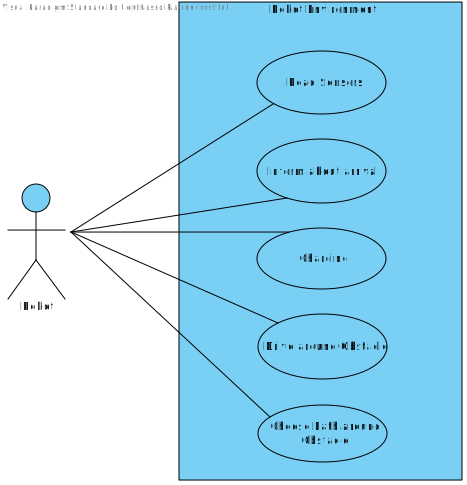
\includegraphics[width=0.8\textwidth]{img/1-Analyse-3-Robot}
				\caption{Use Case Diagramm 1: Use Cases des Roboters}
				\label{fig:3-1-robot-use-cases}
			\end{figure}

			\begin{figure}[H]
				\centering
				\includegraphics[width=0.8\textwidth]{img/1-Analyse-3-Server}
				\caption{Use Case Diagramm 2: Use Cases des Servers}
				\label{fig:3-1-server-use-cases}
			\end{figure}

			\begin{figure}[H]
				\centering
				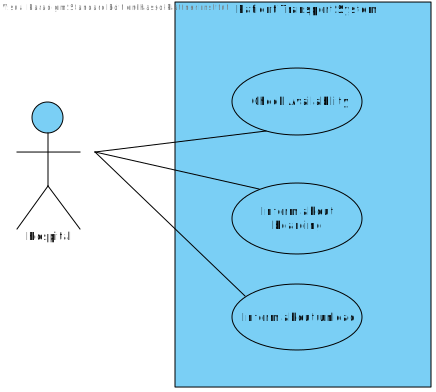
\includegraphics[width=0.8\textwidth]{img/1-Analyse-3-Hospital}
				\caption{Use Case Diagramm 2: Use Cases des Hospitals}
				\label{fig:3-1-hospital-use-cases}
			\end{figure}

		\pagebreak

		\subsection{Beschreibung zu Use Case \emph{1}: Drive to Destination}

			\subsubsection*{Charakterisierende Informationen}

			\begin{table}[H]
				\centering
				\begin{tabularx}{\textwidth}{@{}p{5cm}X@{}}
				\hline
				\textbf{Übergeordneter elementarer Geschäftsprozess:} & Drive to Destination\\ \hline
				\textbf{Ziel des Use Cases:} & \emph{Robot} fährt eine \emph{Destination} an\\ \hline
				\textbf{Umgebende Systemgrenze:} & \emph{Robot} \\ \hline
				\textbf{Vorbedingung:} & Ein spezieller \emph{Robot} wurde vom Server ausgewählt und sein Akkustand ist hoch genug um den Auftrag auszuführen \\ \hline
				\textbf{Nachbedingung bei erfolgreicher Ausführung:} & \emph{Robot} ist an der \emph{Destination} angekommen und meldet dies dem \emph{Server} \\ \hline
				\textbf{Beteiligte Nutzer:} & \emph{Robot} \\ \hline
				\textbf{Auslösendes Ereignis:} & \emph{Robot} hat eine \emph{Destination} erhalten. \\
				\hline
				\end{tabularx}
			\end{table}

			Dieser Use Case wird dann benutzt, wenn ein \emph{Robot} eine aktuelle
			\emph{Destination} hat. In dieser Ausbaustufe betrachten wir lediglich das Anfahren
			einer \emph{Destination} von einem \emph{Robot}. Der \emph{Robot} dreht sich zunächst in die
			Richtung der \emph{Destination} und fährt so lange in Luftlinie, bis er entweder
			ankommt oder ein Hindernis erkennt. Ein konkreter Prozess zur Erkennung
			eines Hindernisses ist eine Entwurfsentscheidung und wird daher noch
			nicht berücksichtigt. Wenn der \emph{Robot} ein \emph{Obstacle} erkennt, dann
			sucht er einen guten Weg um das Hindernis herum. Wie er diesen Weg sucht
			ist auch zunächst eine Entwurfsentscheidung und noch nicht relevant. Auf
			diesem Weg umfährt er dann das \emph{Obstacle} und nimmt erneut die Fahrt auf
			Luftlinie auf.

			\subsubsection*{Szenario für den Standardablauf (Erfolg)}

			\begin{table}[H]
				\centering
				\begin{tabularx}{\textwidth}{@{}cp{2cm}X@{}}
				\hline
				Schritt & Nutzer & Beschreibung der Aktivität \\ \hline
				1 & Robot & \emph{Robot} dreht sich in Richtung aktueller \emph{Destination} \\
				2 & Robot & \emph{Robot} fährt geradeaus \\
				3 & Robot & \emph{Robot} erreicht \emph{Destination} \\
				\hline
				\end{tabularx}
			\end{table}

			\subsubsection*{Szenarien für alternative Abläufe\\ (Misserfolg oder Umwege zum Erfolg)}

			\begin{table}[H]
				\centering
				\begin{tabularx}{\textwidth}{@{}cp{6cm}X@{}}
				\hline
				Schritt & Bedingung für Alternative & Beschreibung der Aktivität \\ \hline
				3 & \emph{Robot} erkennt ein \emph{Obstacle} zwischen auf seinem Weg zum Ziel & \emph{Robot} sucht sich einen Umweg um das \emph{Obstacle}, umfährt das \emph{Obstacle} und nimmt schließlich Standardablauf wieder auf \\
				\hline
				\end{tabularx}
			\end{table}

			%\subsubsection*{Beschreibung des allgemeinen Ablaufes}
			
		\pagebreak

		\subsection{Beschreibung zu Use Case \emph{2}: Read Sensors}

			\subsubsection*{Charakterisierende Informationen}

			\begin{table}[H]
				\centering
				\begin{tabularx}{\textwidth}{@{}p{5cm}X@{}}
				\hline
				\textbf{Übergeordneter elementarer Geschäftsprozess:} & Choose Robot\\ \hline
				\textbf{Ziel des Use Cases:} & \emph{Robot} kann über seinen Akkustand und seine Position Auskunft geben\\ \hline
				\textbf{Umgebende Systemgrenze:} & \emph{Robot} \\ \hline
				\textbf{Vorbedingung:} & \emph{Robot} hat eine Anfrage vom \emph{Server} erhalten \\ \hline
				\textbf{Nachbedingung bei erfolgreicher Ausführung:} & \emph{Robot} schickt die ermittelten Informationen an den \emph{Server} \\ \hline
				\textbf{Beteiligte Nutzer:} & \emph{Robot} \\ \hline
				\textbf{Auslösendes Ereignis:} & \emph{Robot} hat eine Anfrage vom \emph{Server} erhalten, seine Sensoren zu lesen und sie dem \emph{Server} zu schicken \\
				\hline
				\end{tabularx}
			\end{table}

			Im Rahmen vom Geschäftsprozess \emph{Choose Robot} sammelt der \emph{Server}
			Informationen über jeden \emph{Robot}. Diese Informationen (z.B
			Akkustand, aktuelle Position, ob der \emph{Robot} gerade ein Ziel verfolgt)
			kann der \emph{Robot} von seinen Hardware-Schnittstellen anfordern. Dieses
			Use Case wird dann ausgefüht, wenn der \emph{Robot} eine Anfrage vom
			Server erhält, seine Sensoren zu lesen, und endet damit, dass der \emph{Robot}
			die zusammengefassten Informationen an den \emph{Server} schickt.

			\subsubsection*{Szenario für den Standardablauf (Erfolg)}

			\begin{table}[H]
				\centering
				\begin{tabularx}{\textwidth}{@{}cp{2cm}X@{}}
				\hline
				Schritt & Nutzer & Beschreibung der Aktivität \\ \hline
				1 & Robot & \emph{Robot} erhält Anfrage vom \emph{Server} \\
				2 & Robot & \emph{Robot} sammelt Informationen von seiner Hardwareschnittstelle und fasst sie zusammen \\
				3 & Robot & \emph{Robot} schickt zusammengefasste Informationen an den Server \\
				\hline
				\end{tabularx}
			\end{table}

			%\subsubsection*{Beschreibung des allgemeinen Ablaufes}
			
		\pagebreak

		\subsection{Beschreibung zu Use Case \emph{3}: Charging}

			\subsubsection*{Charakterisierende Informationen}

			\begin{table}[H]
				\centering
				\begin{tabularx}{\textwidth}{@{}p{5cm}X@{}}
				\hline
				\textbf{Übergeordneter elementarer Geschäftsprozess:} & Drive to Destination\\ \hline
				\textbf{Ziel des Use Cases:} & Ziel ist es, dem \emph{Robot} zu ermöglichen seine Ladestation anzufahren\\ \hline
				\textbf{Umgebende Systemgrenze:} & \emph{Robot}\\ \hline
				\textbf{Vorbedingung:} & Der \emph{Robot} erreicht sein vorgegebenes Ziel\\ \hline
				\textbf{Nachbedingung bei erfolgreicher Ausführung:} & Der \emph{Robot} erreicht seine Ladestation\\ \hline
				\textbf{Beteiligte Nutzer:} & \emph{Robot}\\ \hline
				\textbf{Auslösendes Ereignis:} & \emph{Robot} erreicht \emph{Destination} (Use-Case)\\
				\hline
				\end{tabularx}
			\end{table}

			Jedem Robot wird, laut Aufgabenstellung, eine feste Ladestation zugewiesen. Der Robot fährt vollständig autonom diese Ladestation an. Daher ist keine Kommunikation mit dem Server notwendig.

			\subsubsection*{Szenario für den Standardablauf (Erfolg)}

			\begin{table}[H]
				\centering
				\begin{tabularx}{\textwidth}{@{}cp{2cm}X@{}}
				\hline
				Schritt & Nutzer & Beschreibung der Aktivität \\ \hline
				1 & Robot & \emph{Robot} erreicht Ziel \\
				2 & Robot & \emph{Robot} fährt zur Ladestation \\
				3 & Robot & \emph{Robot} erreicht Ladestation und lädt sich auf \\
				4 & Robot & \emph{Robot} erhält neues Ziel und fährt dorthin \\
				\hline
				\end{tabularx}
			\end{table}

			%\subsubsection*{Beschreibung des allgemeinen Ablaufes}
			
		\pagebreak
		
			\subsection{Beschreibung zu Use Case \emph{4}: Inform about arrival}

			\subsubsection*{Charakterisierende Informationen}

			\begin{table}[H]
				\centering
				\begin{tabularx}{\textwidth}{@{}p{5cm}X@{}}
				\hline
				\textbf{Übergeordneter elementarer Geschäftsprozess:} & TakePatientToHospital\\ \hline
				\textbf{Ziel des Use Cases:} & Ziel ist es, dem \emph{Robot} zu ermöglichen seine Ankunft dem Krnakenhaus mitzuteilen\\ \hline
				\textbf{Umgebende Systemgrenze:} & \emph{Robot}\\ \hline
				\textbf{Vorbedingung:} & Der \emph{Robot} erreicht die \emph{Position} des Patienten\\ \hline
				\textbf{Nachbedingung bei erfolgreicher Ausführung:} & Der \emph{Robot} wartet bis er beladen wurde\\ \hline
				\textbf{Beteiligte Nutzer:} & \emph{Robot}\\ \hline
				\textbf{Auslösendes Ereignis:} & \emph{Robot} erreicht Patienten\\
				\hline
				\end{tabularx}
			\end{table}

			Der \emph{Robot} erreicht seine vorgegebene \emph{Destination} und muss dem \emph{Hospital} mitteilen, dass er angekommen ist. 

			\subsubsection*{Szenario für den Standardablauf (Erfolg)}

			\begin{table}[H]
				\centering
				\begin{tabularx}{\textwidth}{@{}cp{2cm}X@{}}
				\hline
				Schritt & Nutzer & Beschreibung der Aktivität \\ \hline
				1 & Robot & \emph{Robot} informiert \emph{Server}, dass er angekommen ist.
				\hline
				\end{tabularx}
			\end{table}

			%\subsubsection*{Beschreibung des allgemeinen Ablaufes}
			
		\pagebreak

		\subsection{Beschreibung zu Use Case \emph{5}: Choose Robot}

			\subsubsection*{Charakterisierende Informationen}

			\begin{table}[H]
				\centering
				\begin{tabularx}{\textwidth}{@{}p{5cm}X@{}}
				\hline
				\textbf{Übergeordneter elementarer Geschäftsprozess:} & Choose Robot \\ \hline
				\textbf{Ziel des Use Cases:} & passenden \emph{Robot} für die durch den \emph{Server} gesendete \emph{Destination} auswählen\\ \hline
				\textbf{Umgebende Systemgrenze:} & \emph{Robot} und \emph{Server} \\ \hline
				\textbf{Vorbedingung:} & \emph{Server} hat eine neue \emph{Destination} bekommen\\ \hline
				\textbf{Nachbedingung bei erfolgreicher Ausführung:} & dem ausgewählten \emph{Robot} wird die Task übertragen\\ \hline
				\textbf{Beteiligte Nutzer:} & \emph{Robot} und \emph{Server}\\ \hline
				\textbf{Auslösendes Ereignis:} & \emph{Server} empfängt neue \emph{Destination}\\
				\hline
				\end{tabularx}
			\end{table}

			\subsubsection*{Szenario für den Standardablauf (Erfolg)}

			\begin{table}[H]
				\centering
				\begin{tabularx}{\textwidth}{@{}cp{2cm}X@{}}
				\hline
				Schritt & Nutzer & Beschreibung der Aktivität \\ \hline
				1 & Server & \emph{Server} sendet Anfragen an alle \emph{Robots} \\
				2 & Robot & \emph{Robots} empfangen Anfrage und führen dann den Use-Case „read Sensor“ aus \\
				3 & Robot & \emph{Robots} senden ihre ermittelten Sensorwerte an den \emph{Server}\\
				4 & Server & \emph{Server} empfängt Daten und wählt den am Besten geeigneten \emph{Robot} aus \\
				\hline
				\end{tabularx}
			\end{table}

			%\subsubsection*{Beschreibung des allgemeinen Ablaufes}
			
		\pagebreak

		\subsection{Beschreibung zu Use Case \emph{6}: Assign Task}

			\subsubsection*{Charakterisierende Informationen}

			\begin{table}[H]
				\centering
				\begin{tabularx}{\textwidth}{@{}p{5cm}X@{}}
				\hline
				\textbf{Übergeordneter elementarer Geschäftsprozess:} & Choose Robot  \\ \hline
				\textbf{Ziel des Use Cases:} & \emph{Robot} den Task (die \emph{Destination}) zuweisen\\ \hline
				\textbf{Umgebende Systemgrenze:} & \emph{Server} und \emph{Robot} \\ \hline
				\textbf{Vorbedingung:} & „Choose Robot“ hat am Besten geeigneten \emph{Robot} gefunden und ausgewählt\\ \hline
				\textbf{Nachbedingung bei erfolgreicher Ausführung:} & Ausgewählter \emph{Robot} steuert die \emph{Destination} an\\ \hline
				\textbf{Beteiligte Nutzer:} & \emph{Server} und \emph{Robot}\\ \hline
				\textbf{Auslösendes Ereignis:} & Im Use-Case „choose Robot“ wurde passender \emph{Robot} ausgewählt\\
				\hline
				\end{tabularx}
			\end{table}
			
			Dem \emph{Server} wird hiermit die Möglichkeit gegeben, dem \emph{Robot} eine beliebige \emph{Destination} zuzuweisen. 

			\subsubsection*{Szenario für den Standardablauf (Erfolg)}

			\begin{table}[H]
				\centering
				\begin{tabularx}{\textwidth}{@{}cp{2cm}X@{}}
				\hline
				Schritt & Nutzer & Beschreibung der Aktivität \\ \hline
				1 & Server & \emph{Server} überträgt ausgewähltem \emph{Robot} den Task \\
				\hline
				\end{tabularx}
			\end{table}

			%\subsubsection*{Beschreibung des allgemeinen Ablaufes}

	\pagebreak


		\subsection{Beschreibung zu Use Case \emph{7}: Check Availability}

			\subsubsection*{Charakterisierende Informationen}

			\begin{table}[H]
				\centering
				\begin{tabularx}{\textwidth}{@{}p{5cm}X@{}}
				\hline
				\textbf{Übergeordneter elementarer Geschäftsprozess:} & TakePatientToHospital  \\ \hline
				\textbf{Ziel des Use Cases:} & \emph{Hospital} erfährt, ob ein Auftrag vom System entgegengenommen werden kann. \hline
				\textbf{Umgebende Systemgrenze:} &  \\ \hline
				\textbf{Vorbedingung:} &  \hline
				\textbf{Nachbedingung bei erfolgreicher Ausführung:} & Das System führt den Auftrag aus und bringt den \emph{Patient} in das \emph{Hospital} \\ \hline
				\textbf{Beteiligte Nutzer:} & \emph{Hospital} und \emph{Server}\\ \hline
				\textbf{Auslösendes Ereignis:} & \emph{Hospital} hat einen neuen Auftrag\\
				\hline
				\end{tabularx}
			\end{table}

			Das \emph{Hospital} fragt laut Aufgabenstellung an dem zu modellierenden System an, ob ein \emph{Robot} verfügbar ist, um einen \emph{Patient} anzufahren und ins \emph{Hospital} zu bringen. Dazu wird vom \emph{Server} unter anderem der Use Case \emph{Choose Robot} ausgeführt. Es kann passieren, dass kein \emph{Robot} verfügbar ist, dann soll wie in der Aufgabenstellung beschrieben der Auftrag vom System abgelehnt werden. Was das \emph{Hospital} dann für Maßnahmen ergreift, wird hier nicht modelliert da es nicht teil des Systems ist.

			%\subsubsection*{Beschreibung des allgemeinen Ablaufes}

	\pagebreak
		\subsection{Beschreibung zu Use Case \emph{8}: Inform about boarding}

			\subsubsection*{Charakterisierende Informationen}

			\begin{table}[H]
				\centering
				\begin{tabularx}{\textwidth}{@{}p{5cm}X@{}}
				\hline
				\textbf{Übergeordneter elementarer Geschäftsprozess:} & TakePatientToHospital   \\ \hline
				\textbf{Ziel des Use Cases:} & Dem \emph{Robot} mitteilen, dass Patient auf den \emph{Robot} beladen wurde \\ \hline
				\textbf{Umgebende Systemgrenze:} & \emph{Hospital} \\ \hline
				\textbf{Vorbedingung:} & Patient befindet sich auf \emph{Robot}\\ \hline
				\textbf{Nachbedingung bei erfolgreicher Ausführung:} & \emph{Robot} fährt Patienten zum \emph{Hospital} \\ \hline
				\textbf{Beteiligte Nutzer:} & \emph{Hospital}\\ \hline
				\textbf{Auslösendes Ereignis:} & \emph{Server} wurde informiert, dass \emph{Robot} am Patienten angekommen ist(Inform about arrival)\\
				\hline
				\end{tabularx}
			\end{table}
			
			Das \emph{Hospital} muss dem \emph{Robot} mitteilen, dass der Patient beladen wurde um einen sicheren Transport des Patienten zu gewährleisten. Der \emph{Robot} hat somit keinen Eingriff in das Beladen des Patienten.

			\subsubsection*{Szenario für den Standardablauf (Erfolg)}

			\begin{table}[H]
				\centering
				\begin{tabularx}{\textwidth}{@{}cp{2cm}X@{}}
				\hline
				Schritt & Nutzer & Beschreibung der Aktivität \\ \hline
				1 & \emph{Hospital} & Patient wird auf Roboter beladen \\
				2 & \emph{Hospital} & \emph{Hospital} sendet Nachricht an Server, dass sich Patient auf dem \emph{Robot} befindet \\
				\hline
				\end{tabularx}
			\end{table}

			%\subsubsection*{Beschreibung des allgemeinen Ablaufes}

	\pagebreak


\section{Produktumgebung}

  \subsection{Systemumgebung}
  Im nachfolgenden Abschnitt werden die bekannten Komponenten des Systems
  und die dazugehörigen Schnittstellen beschrieben. 
  Grundsätzlich besteht
  das System aus mindestens einem \emph{Robot}, hierfür geeigneten
  \emph{Chargern} und einem zentralen \emph{Server}.

  \subsubsection{Hardwareumgebung}

  \paragraph{Server}\label{server}

  Es existiert ein zentraler \emph{Server}, der über ausreichende Ressourcen verfügt. 
  Dieser \emph{Server} besitzt einen zentralen Hauptprozessor, über den er auf alle weiteren Komponenten zugreifen kann kann. 
  Zu diesen Komponenten zählen der \emph{NetworkAccess}, über welchen, der \emph{Server} auf das Funknetzwerk zugreifen kann. 
  Über dieses Funknetzwerk können alle \emph{RobotUnits} erreicht werden, sodass Nachrichten an sie abgesetzt werden können und Nachrichten, die über das Funknetzwerk für den \emph{Server} übertragen wurden, empfangen werden können. 
  Über eine weitere Komponente kann der \emph{Server} mit dem zentralen \emph{Hospital} kommunizieren. 
  Dies schließt das Senden und das Empfangen von Nachrichten in beiden Richtungen ein. 
  Die Kommunikation mit den Kunden der Taxi-App wird ebenfalls über eine gesonderte Komponente mit ähnlicher Funktionalität realisiert.

  \paragraph{RobotUnit}\label{robotunit}

  Das Transportvehikel \emph{RobotUnit} stellt die Kernkomponente der Hardwareumgebung dar. 
  Über einen zentralen Hauptprozessor kann dieses auf alle weiteren Komponenten zugreifen. 
  Als Antrieb nutzt das Transportvehikel die \emph{IRobotEngine}: einen omnidirektionalen Antrieb mit 3 Motoren, über welchen es sich vorwärts, nach rechts, nach links oder durch Drehen um die eigene Achse bewegen lässt. 
  Der Antrieb ermöglicht eine Fahrt in verschiedenen Geschwindigkeiten. 
  Die \emph{RobotUnit} verfügt außerdem über 9 Infarotdistanzsensoren, die an der kreisförmigen Außenwand des Vehikels im Abstand von jeweils 40 Grad angeordnet sind. 
  Über sie ist die Feststellung der Entfernung des Vehikels von allen bewegten und unbewegten Objekten in der Umgebung möglich. 
  Bei einer Kollision der \emph{RobotUnit} mit einem anderen Objekt wird dieses Ereignis über die Sensorik einer Kollisionserkennung festgestellt, worauf weitere Schritte eingeleitet werden können. 
  Über ein GPS-Modul kann die aktuelle Lage und Ausrichtung der \emph{RobotUnit} ermittelt werden. 
  Zur Ermöglichung von Kommunikation besitzt die \emph{RobotUnit} ein Wlan-Modul, über welches Nachrichten über ein zur Verfügung stehendendes Funknetzwerk gesendet und empfangen werden können. 
  Jede \emph{RobotUnit} verfügt über einen Akkumulator, der zur Energieversorgung dient. 
  Eine ausreichende Ladung des Akkumulators ist deshalb zum Betrieb der \emph{RobotUnit} unbedingt erforderlich. 
  Der Akkumulator hat eine maximale Ladekapazität und kann über einen \emph{Charger} geladen werden. 
  Zur genauen Beschaffenheit des Akkumulators ist nichts bekannt.

  \paragraph{Charger}\label{charger}

  Es existieren Ladestationen, über die sich der Akkumulator der\emph{RobotUnit} vollständig laden lässt. 
  Eine Ladestation ist dabei genau einer \emph{RobotUnit} zugeordnet. 
  Zum Laden muss eine \emph{RobotUnit} seine Ladestation anfahren, worauf die Ladung sofort beginnt. 
  Jede Ladestation verfügt über eine genaue Position.

    \subsubsection{Softwareumgebung}

    \paragraph{Server}\label{server}
    		Auf dem \emph{Server} läuft, da nicht anders angegeben, ein Standard-Betriebssystem. 
    		Darauf läuft eine Laufzeitumgebung, die die benötigten Methoden zur Kommunikation mit den \emph{Robots} bereitstellt. 
    		Die wichtigste (und einzige bisher spezifizierte) Methode, ist die CallRobot() Methode um einen \emph{Robot} anzurufen und einen Datenaustausch herzustellen.
    	\subparagraph{IServerWlanAdapter}\label{iserverwlanadapter}
    		Der \emph{IServerWlanAdapter} ist die Komponente des \emph{Servers}, mit der er die Verbindung zum \emph{Robot} herstellt. Hierüber werden Nachrichten ausgetauscht. 
    		Dementsprechend stehen Methoden zum Senden einer Message, registrieren eines IMessageHandlers, auslesen von NetworkIDs usw. bereit.
    	\subparagraph{IHospital}\label{ihospital}
    		Bei \emph{IHospital} handelt es sich um die \emph{Server} Komponente, die die Kommunikation mit dem \emph{Hospital} gewährleistet. 
    		Dabei werden zum einen Methoden bereitgestellt, die das \emph{Hospital} über ein Interface aufrufen kann, um Aufträge zu verteilen und dem \emph{Hospital} Informationen über den aktuellen Stand des Auftrags mitzuteilen (getPatientAt(), patientOnBoard() sowie patientArrived()), und zum anderen kann die Komponente über ein Interface Methoden des \emph{Hospitals} aufrufen, um diesem Informationen zu übermitteln (informRobotArrivedAtPatient() und informRobotArrivedAtHospital()).
      \subparagraph{ITaxiApp}
      Die \emph{ITaxiApp} Komponente ist ein Contatiner, über den die Kommunikation des Servers mit den Apps der Benutzer der nicht-modellierten mobilen Taxi-Applikation realisiert wird. 
      Der Container stellt ein Taxi-App Objekt für jeden Benutzer bereit. 
      Die Kommunikation findet über mehrere Schnittstellen statt. 
      Über das IAppContainer Interface, kann der Server Taxi-App Objekte bekommen. 
      Über die Interfaces ITaxiAppUserOutput und ITaxiAppUserInputHandler kann der Server mit den einzelnen Apps und damit mit den Kunden kommunizieren. 
      Das ITaxiApp Interface stellt die Methoden zum Zugriff aud die Kommunikationsinterfaces, sowie eine Methode zur Ermittlung der App-ID bereit.
Robot
    \paragraph{Robot}\label{robot}
    		Nachfolgend werden die zentralen Softwareschnittstellen des \emph{Robots} beschrieben.
    	\subparagraph{IRobotCore}\label{irobotcore}
    		Auf der zentralen Recheneinheit des \emph{Robots}, dem \emph{IRobotCore}, läuft eine JavaRuntimeEnvironment, in der sich die gesamte Steuerung und die Verwendung der Komponenten und Schnittstellen abspielt. 
    		Die einzelnen Komponenten mit ihren Methoden werden im folgenden näher erläutert.
    	\subparagraph{IRSensorDistance}\label{irsensordistance}
    		Die \emph{IRSensorDistance} Komponente stellt drei Methoden bereit, mit denen die Distanz und der Winkel des entdeckten Objekts und der an der Entdeckung beteiligte Infrarotsensor erfasst und in Arrays gespeichert werden.
    	\subparagraph{IDistanceSensor}\label{idistancesensor}
    		Die besagten Arrays kann der \emph{IDistanceSensor} auslesen. 
    		Er hat dazu ebenfalls drei Methoden. getIRDistances() gibt ein Array mit allen erfassten Objekten zurück, getIRDistancesInRange() gibt ebenfalls ein Array zurück, das allerdings nur die Objekte in einem gewissen Abstand enthält und getNearestIRDistances() gibt nur das nächste Objekt zurück.
    	\subparagraph{INorthStar}\label{inorthstar}
    		Die Komponente \emph{INorthStar} ist für die Positionierung zuständig und greift dabei auf ein Device zur Standortbestimmung zurück. 
    		Sie hat zwei Methoden. 
    		Eine liest die aktuelle Position aus, die andere die aktuelle Ausrichtung. 
    		Die Position besteht dabei aus zwei float-Werten, einer x- und einer y-Koordinate.
    	\subparagraph{IRobotWlanAdapter}\label{irobotwlanadapter}
    		Bei \emph{IRobotWlanAdapter} handelt es sich um die Komponente, mit der auf Seite des \emph{Robots} die Kommunikation zwischen \emph{Robot} und \emph{Server} ermöglicht wird. 
    		Entsprechend gibt es hier die gleichen Methoden zur Kommunikation, die auch die \emph{IServerWlanAdapter} Komponente bereitstellt.
    	\subparagraph{IBumperHandler}\label{ibumperhandler}
    		\emph{IBumperHandler} ist die Komponente zum Umgang mit Zusammenstößen. 
    		Die Kollisionserkennung IBumper registriert einen Aufprall und die \emph{IBumperHandler} Komponente stellt zwei Methoden zum Umgang mit dem Aufprall bereit.
    	\subparagraph{IDrive}\label{idrive}
    		Die Bewegungssteuerung des \emph{Robots} heißt \emph{IDrive}. 
    		Sie stellt vier Methoden bereit. 
    		Die Methoden driveToPosition() und driveToPositionCautiously() erwarten beide eine Position, eine Geschwindigkeit und einen ArrivalHandler, der eine Methode zur Meldung aufruft, wenn der \emph{Robot} am Ziel angekommen ist. 
    		Die Methoden sind beide dafür da, ein gegebenes Ziel anzufahren, wobei bei der Zweiten die Höchstgeschwindigkeit geringer ist.
    		 Die Höchstgeschwindigkeit für Cautiously, Regular und Fast Methoden stellt die \emph{IDrive} Komponente bereit, wobei Cautiously $\leq$ Regular $\leq$ Fast gilt. 
    		 Die anderen beiden Methoden, drive() und driveCautiously() unterscheiden sich ebenfalls nur in der Höchstgeschwindigkeit und ermöglichen ein manuelles Fahren. 
    		 Dabei erwarten sie die Drehung des \emph{Robots} als float-Wert sowie die Vorwärts- und die Seitwärtsgeschwindigkeit, ebenfalls als float-Wert.
    	\subparagraph{IBattery}\label{ibattery}
    		Bei \emph{IBattery} handelt es sich um die Akkusteuerung des \emph{Robots}. 
    		Sie stellt zwei Methoden bereit. 
    		getBatteryLevel() gibt den aktuellen Akkuladestand als float-Wert zurück, getChargingPosition() gibt die Position des zugeordneten Chargers zurück.


\pagebreak
\subsubsection{Ressourcenübersicht}
    In Abbildung \ref{fig:4-1-3-verteilungsdiagramm} werden die in 4.1.1 und 4.1.2 beschriebenen
    Komponenten und Schnittstellen im Verteilungsdiagramm dargestellt.

    \begin{figure}[H]
      \centering
      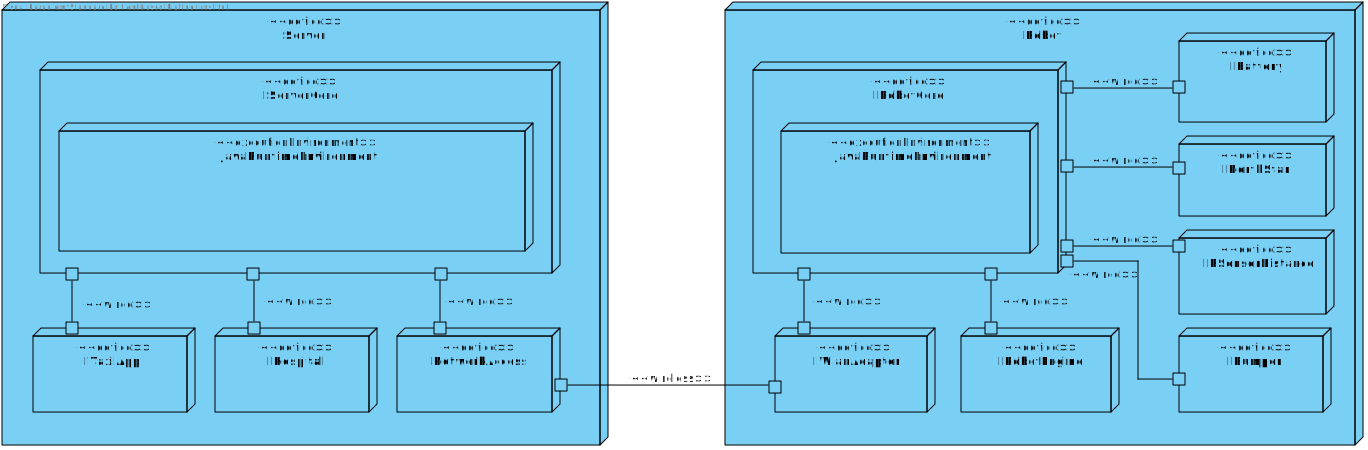
\includegraphics[width=1.2\textwidth, angle=90]{img/2-Analyse-4-Produktumgebung}
      \caption{Verteilungsdiagramm}
      \label{fig:4-1-3-verteilungsdiagramm}
    \end{figure}


\end{document}
